\documentclass{standalone}
\usepackage{tikz}
\usetikzlibrary{patterns, positioning}


\begin{document}
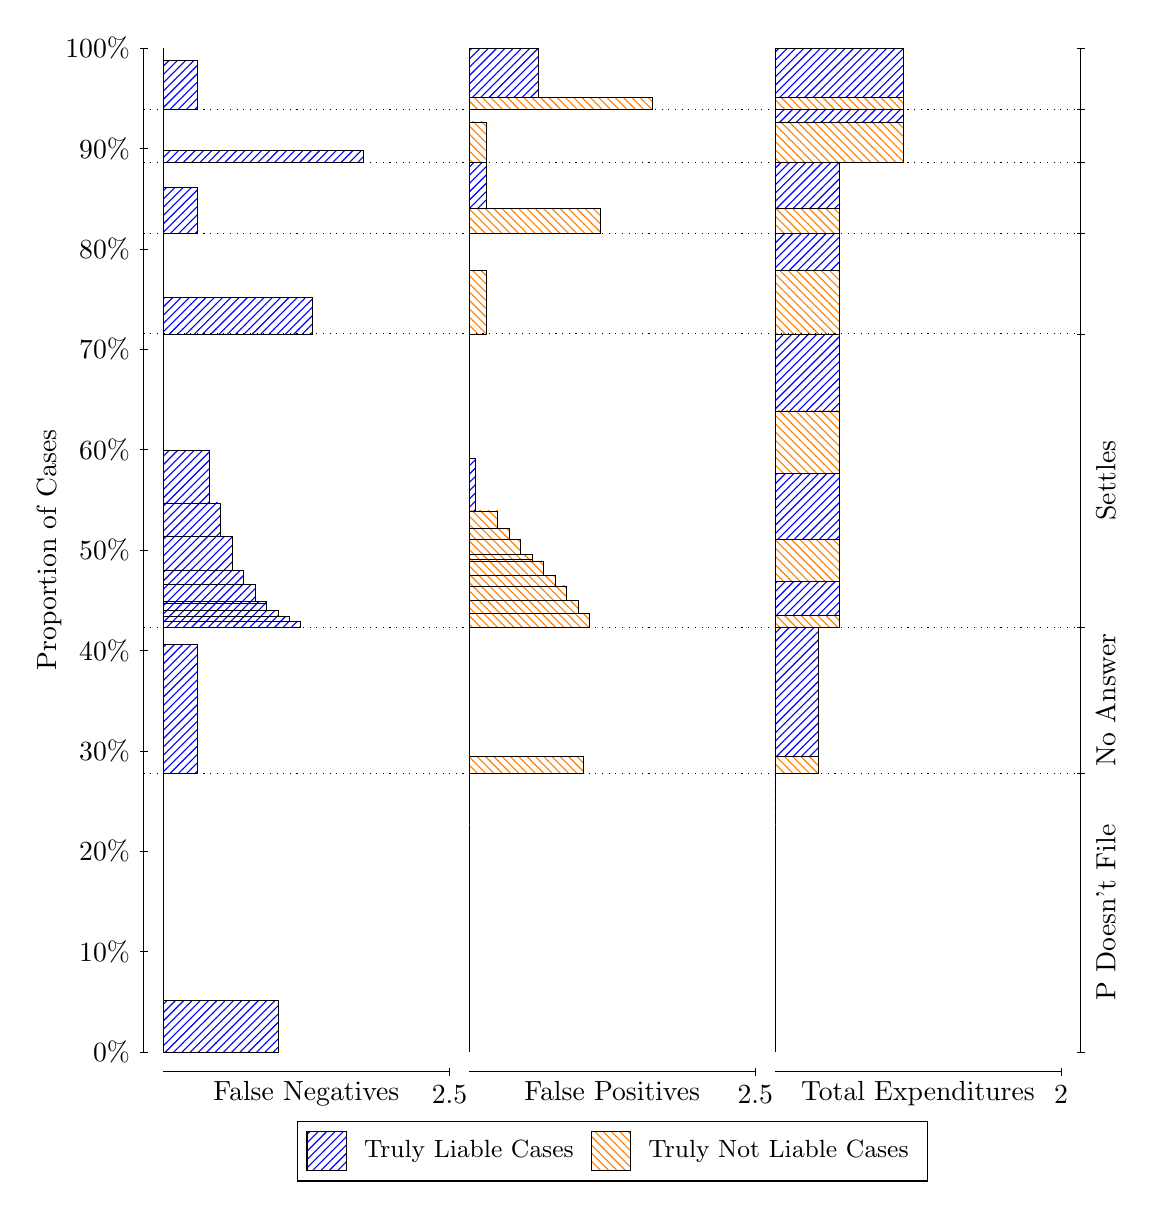
\begin{tikzpicture}
\draw[black, very thin] (1.5,1.75) -- (1.5,14.5);
\node[rotate=90, text=black, anchor=center] at (0.3, 8.125) {Proportion of Cases};
\draw[black, very thin] (1.45,1.75) -- (1.55,1.75);
\node[text=black, anchor=east] at (1.45, 1.75) {0\%};
\draw[black, very thin] (1.45,3.025) -- (1.55,3.025);
\node[text=black, anchor=east] at (1.45, 3.025) {10\%};
\draw[black, very thin] (1.45,4.3) -- (1.55,4.3);
\node[text=black, anchor=east] at (1.45, 4.3) {20\%};
\draw[black, very thin] (1.45,5.575) -- (1.55,5.575);
\node[text=black, anchor=east] at (1.45, 5.575) {30\%};
\draw[black, very thin] (1.45,6.85) -- (1.55,6.85);
\node[text=black, anchor=east] at (1.45, 6.85) {40\%};
\draw[black, very thin] (1.45,8.125) -- (1.55,8.125);
\node[text=black, anchor=east] at (1.45, 8.125) {50\%};
\draw[black, very thin] (1.45,9.4) -- (1.55,9.4);
\node[text=black, anchor=east] at (1.45, 9.4) {60\%};
\draw[black, very thin] (1.45,10.675) -- (1.55,10.675);
\node[text=black, anchor=east] at (1.45, 10.675) {70\%};
\draw[black, very thin] (1.45,11.95) -- (1.55,11.95);
\node[text=black, anchor=east] at (1.45, 11.95) {80\%};
\draw[black, very thin] (1.45,13.225) -- (1.55,13.225);
\node[text=black, anchor=east] at (1.45, 13.225) {90\%};
\draw[black, very thin] (1.45,14.5) -- (1.55,14.5);
\node[text=black, anchor=east] at (1.45, 14.5) {100\%};

\draw[black, very thin] (13.4,1.75) -- (13.4,14.5);
\draw[black, very thin] (13.35,1.75) -- (13.45,1.75);
\node[anchor=west] at (13.35, 1.75) {};
\draw[black, very thin] (13.35,5.2917) -- (13.45,5.2917);
\node[anchor=west] at (13.35, 5.2917) {};
\draw[black, very thin] (13.35,7.1424) -- (13.45,7.1424);
\node[anchor=west] at (13.35, 7.1424) {};
\draw[black, very thin] (13.35,10.87) -- (13.45,10.87);
\node[anchor=west] at (13.35, 10.87) {};
\draw[black, very thin] (13.35,12.142) -- (13.45,12.142);
\node[anchor=west] at (13.35, 12.142) {};
\draw[black, very thin] (13.35,13.048) -- (13.45,13.048);
\node[anchor=west] at (13.35, 13.048) {};
\draw[black, very thin] (13.35,13.716) -- (13.45,13.716);
\node[anchor=west] at (13.35, 13.716) {};
\draw[black, very thin] (13.35,14.5) -- (13.45,14.5);
\node[anchor=west] at (13.35, 14.5) {};

\draw[black, very thin, pattern color=blue, pattern=north east lines] (1.75,1.75) rectangle (3.2033,2.4006);
\draw[black, very thin, pattern color=orange, pattern=north west lines] (1.75,2.4006) rectangle (1.75,5.2917);
\draw[black, very thin, pattern color=blue, pattern=north east lines] (1.75,5.2917) rectangle (2.186,6.9295);
\draw[black, very thin, pattern color=orange, pattern=north west lines] (1.75,6.9295) rectangle (1.75,7.1424);
\draw[black, very thin, pattern color=blue, pattern=north east lines] (1.75,7.1424) rectangle (3.494,7.2225);
\draw[black, very thin, pattern color=blue, pattern=north east lines] (1.75,7.2225) rectangle (3.3487,7.2818);
\draw[black, very thin, pattern color=blue, pattern=north east lines] (1.75,7.2818) rectangle (3.2033,7.3604);
\draw[black, very thin, pattern color=blue, pattern=north east lines] (1.75,7.3604) rectangle (3.058,7.4523);
\draw[black, very thin, pattern color=blue, pattern=north east lines] (1.75,7.4523) rectangle (3.058,7.4741);
\draw[black, very thin, pattern color=blue, pattern=north east lines] (1.75,7.4741) rectangle (2.9127,7.6903);
\draw[black, very thin, pattern color=blue, pattern=north east lines] (1.75,7.6903) rectangle (2.7673,7.8618);
\draw[black, very thin, pattern color=blue, pattern=north east lines] (1.75,7.8618) rectangle (2.622,8.293);
\draw[black, very thin, pattern color=blue, pattern=north east lines] (1.75,8.293) rectangle (2.4767,8.7221);
\draw[black, very thin, pattern color=blue, pattern=north east lines] (1.75,8.7221) rectangle (2.3313,9.3902);
\draw[black, very thin, pattern color=orange, pattern=north west lines] (1.75,9.3902) rectangle (1.75,10.87);
\draw[black, very thin, pattern color=blue, pattern=north east lines] (1.75,10.87) rectangle (3.6393,11.338);
\draw[black, very thin, pattern color=orange, pattern=north west lines] (1.75,11.338) rectangle (1.75,12.142);
\draw[black, very thin, pattern color=blue, pattern=north east lines] (1.75,12.142) rectangle (2.186,12.729);
\draw[black, very thin, pattern color=orange, pattern=north west lines] (1.75,12.729) rectangle (1.75,13.048);
\draw[black, very thin, pattern color=blue, pattern=north east lines] (1.75,13.048) rectangle (4.2933,13.202);
\draw[black, very thin, pattern color=orange, pattern=north west lines] (1.75,13.202) rectangle (1.75,13.716);
\draw[black, very thin, pattern color=blue, pattern=north east lines] (1.75,13.716) rectangle (2.186,14.346);
\draw[black, very thin, pattern color=orange, pattern=north west lines] (1.75,14.346) rectangle (1.75,14.5);
\draw[black, very thin, pattern color=orange, pattern=north west lines] (5.6333,1.75) rectangle (5.6333,4.6411);
\draw[black, very thin, pattern color=blue, pattern=north east lines] (5.6333,4.6411) rectangle (5.6333,5.2917);
\draw[black, very thin, pattern color=orange, pattern=north west lines] (5.6333,5.2917) rectangle (7.0867,5.5046);
\draw[black, very thin, pattern color=blue, pattern=north east lines] (5.6333,5.5046) rectangle (5.6333,7.1424);
\draw[black, very thin, pattern color=orange, pattern=north west lines] (5.6333,7.1424) rectangle (7.1593,7.3247);
\draw[black, very thin, pattern color=orange, pattern=north west lines] (5.6333,7.3247) rectangle (7.014,7.4816);
\draw[black, very thin, pattern color=orange, pattern=north west lines] (5.6333,7.4816) rectangle (6.8687,7.6686);
\draw[black, very thin, pattern color=orange, pattern=north west lines] (5.6333,7.6686) rectangle (6.7233,7.8068);
\draw[black, very thin, pattern color=orange, pattern=north west lines] (5.6333,7.8068) rectangle (6.578,7.98);
\draw[black, very thin, pattern color=orange, pattern=north west lines] (5.6333,7.98) rectangle (6.4327,8.0086);
\draw[black, very thin, pattern color=orange, pattern=north west lines] (5.6333,8.0086) rectangle (6.4327,8.0741);
\draw[black, very thin, pattern color=orange, pattern=north west lines] (5.6333,8.0741) rectangle (6.2873,8.2639);
\draw[black, very thin, pattern color=orange, pattern=north west lines] (5.6333,8.2639) rectangle (6.142,8.3952);
\draw[black, very thin, pattern color=orange, pattern=north west lines] (5.6333,8.3952) rectangle (5.9967,8.6223);
\draw[black, very thin, pattern color=blue, pattern=north east lines] (5.6333,8.6223) rectangle (5.706,9.2905);
\draw[black, very thin, pattern color=blue, pattern=north east lines] (5.6333,9.2905) rectangle (5.6333,10.87);
\draw[black, very thin, pattern color=orange, pattern=north west lines] (5.6333,10.87) rectangle (5.8513,11.674);
\draw[black, very thin, pattern color=blue, pattern=north east lines] (5.6333,11.674) rectangle (5.6333,12.142);
\draw[black, very thin, pattern color=orange, pattern=north west lines] (5.6333,12.142) rectangle (7.3047,12.461);
\draw[black, very thin, pattern color=blue, pattern=north east lines] (5.6333,12.461) rectangle (5.8513,13.048);
\draw[black, very thin, pattern color=orange, pattern=north west lines] (5.6333,13.048) rectangle (5.8513,13.563);
\draw[black, very thin, pattern color=blue, pattern=north east lines] (5.6333,13.563) rectangle (5.6333,13.716);
\draw[black, very thin, pattern color=orange, pattern=north west lines] (5.6333,13.716) rectangle (7.9587,13.87);
\draw[black, very thin, pattern color=blue, pattern=north east lines] (5.6333,13.87) rectangle (6.5053,14.5);
\draw[black, very thin, pattern color=orange, pattern=north west lines] (9.5167,1.75) rectangle (9.5167,4.6411);
\draw[black, very thin, pattern color=blue, pattern=north east lines] (9.5167,4.6411) rectangle (9.5167,5.2917);
\draw[black, very thin, pattern color=orange, pattern=north west lines] (9.5167,5.2917) rectangle (10.062,5.5046);
\draw[black, very thin, pattern color=blue, pattern=north east lines] (9.5167,5.5046) rectangle (10.062,7.1424);
\draw[black, very thin, pattern color=orange, pattern=north west lines] (9.5167,7.1424) rectangle (10.334,7.2992);
\draw[black, very thin, pattern color=blue, pattern=north east lines] (9.5167,7.2992) rectangle (10.334,7.7283);
\draw[black, very thin, pattern color=orange, pattern=north west lines] (9.5167,7.7283) rectangle (10.334,8.2553);
\draw[black, very thin, pattern color=blue, pattern=north east lines] (9.5167,8.2553) rectangle (10.334,9.096);
\draw[black, very thin, pattern color=orange, pattern=north west lines] (9.5167,9.096) rectangle (10.334,9.8921);
\draw[black, very thin, pattern color=blue, pattern=north east lines] (9.5167,9.8921) rectangle (10.334,10.87);
\draw[black, very thin, pattern color=orange, pattern=north west lines] (9.5167,10.87) rectangle (10.334,11.674);
\draw[black, very thin, pattern color=blue, pattern=north east lines] (9.5167,11.674) rectangle (10.334,12.142);
\draw[black, very thin, pattern color=orange, pattern=north west lines] (9.5167,12.142) rectangle (10.334,12.461);
\draw[black, very thin, pattern color=blue, pattern=north east lines] (9.5167,12.461) rectangle (10.334,13.048);
\draw[black, very thin, pattern color=orange, pattern=north west lines] (9.5167,13.048) rectangle (11.152,13.563);
\draw[black, very thin, pattern color=blue, pattern=north east lines] (9.5167,13.563) rectangle (11.152,13.716);
\draw[black, very thin, pattern color=orange, pattern=north west lines] (9.5167,13.716) rectangle (11.152,13.87);
\draw[black, very thin, pattern color=blue, pattern=north east lines] (9.5167,13.87) rectangle (11.152,14.5);
\draw[black, dotted] (1.5,5.2917) -- (13.4,5.2917);
\draw[black, dotted] (1.5,7.1424) -- (13.4,7.1424);
\draw[black, dotted] (1.5,10.87) -- (13.4,10.87);
\draw[black, dotted] (1.5,12.142) -- (13.4,12.142);
\draw[black, dotted] (1.5,13.048) -- (13.4,13.048);
\draw[black, dotted] (1.5,13.716) -- (13.4,13.716);
\draw[black, very thin] (1.75,1.5) -- (5.3833,1.5);
\node[text=black, anchor=north] at (3.5667, 1.5) {False Negatives};
\draw[black, very thin] (5.3833,1.45) -- (5.3833,1.55);
\node[text=black, anchor=north] at (5.3833, 1.45) {2.5};

\draw[black, very thin] (5.6333,1.5) -- (9.2667,1.5);
\node[text=black, anchor=north] at (7.45, 1.5) {False Positives};
\draw[black, very thin] (9.2667,1.45) -- (9.2667,1.55);
\node[text=black, anchor=north] at (9.2667, 1.45) {2.5};

\draw[black, very thin] (9.5167,1.5) -- (13.15,1.5);
\node[text=black, anchor=north] at (11.333, 1.5) {Total Expenditures};
\draw[black, very thin] (13.15,1.45) -- (13.15,1.55);
\node[text=black, anchor=north] at (13.15, 1.45) {2};

\node[text=black, centered, rotate=90] at (13.72, 3.5208) {P Doesn't File};
\node[text=black, centered, rotate=90] at (13.72, 6.217) {No Answer};
\node[text=black, centered, rotate=90] at (13.72, 9.0063) {Settles};





\draw (7.449999999999999,1.5) node[draw=none] (baseCoordinate) {};
\begin{scope}[align=center]
        \matrix[scale=0.5, draw=black, below=0.5cm of baseCoordinate, nodes={draw}, column sep=0.1cm]{
            \node[rectangle, draw, minimum width=0.5cm, minimum height=0.5cm, pattern color=blue, pattern=north east lines] {}; &
            \node[draw=none, font=\small, text=black] (B) {Truly Liable Cases}; &
            \node[rectangle, draw, minimum width=0.5cm, minimum height=0.5cm, pattern color=orange, pattern=north west lines] {}; &
            \node[draw=none, font=\small, text=black] (B) {Truly Not Liable Cases}; \\
            };
\end{scope}

\end{tikzpicture}
\end{document}